\documentclass{article}
\usepackage{graphicx}
\usepackage{url}
%\usepackage{hyperref}
\usepackage{verbatim}
%\usepackage{times,mathptm}
\usepackage{times}
% the following package is optional:
%\usepackage{latexsym}
%\usepackage{picins}
\usepackage{url}
\usepackage{epsfig}
\usepackage{amsmath}
%\usepackage{macros}
%\usepackage{small-caption}
%\usepackage[l]{floatflt}

\begin{document}

\title{Technical Challenges for the RoboCup 2010 Standard Platform League Competition}

\author{RoboCup SPL Technical Committee}

\maketitle

\section{Introduction}
\label{sec:introduction}

There are three technical challenges that will be held at the RoboCup 
2010 Standard Platform League Competition. These are:

\begin{itemize}
\item The Open Challenge (Section~\ref{sec:open})
\item The Passing Challenge (Section~\ref{sec:passing})
\item The Dribbling Challenge (Section~\ref{sec:dribbling})
\end{itemize}

The team with the top score in a challenge will receive 25 points, each 
position thereafter will receive 1 less point; i.e. 1st = 25pt, 2nd = 24pts, 
3rd = 23pts ... 25th = 1pts. In the case of a draw, each team will receive 
the average of the points allocated to these positions; e.g. if three team 
tie for 2nd, they will receive $(24+23+22)/3 = 23$ points. Teams not competing 
in a challenge will receive 0 points, also if a team competes but fails to 
score a point (or receive a vote) they will receive 0 points again. The team 
with the highest total score after all challenges is deemed the overall 
challenge winner.

All challenges will use the 2010 field and the 2010 rules will apply.

The challenges will be performed separately in three two hour time slots. 
In each time slot, five minutes are reserved for each team, \emph{three minutes} 
of which will be used for the actual challenge. The remaining two minutes are 
reserved for setup and intermediate stoppages if the challenge requires them.

Ten minutes before each Technical Challenge two hour time slot starts, the teams 
have to provide the robots participating in the challenge to the Technical Committee 
(switched off).

Before each challenge, the robot(s) will be booted and put into the \emph{penalized} 
state. For the start of the challenge they will be unpenalized, either by the 
GameController or manually by pushing the chest button. The GameController will 
configure the robots to team color \emph{blue}.

\textbf{Important Note:} \emph{Participation in at least 2 of the 3 challenges and 
receiving more than 0 points in both is required for a team to be considered as 
a pre-qualified team candidate. If a team fails in the challenges or does not 
participate at all, that team will not be considered for pre-qualification even 
if it does well in the soccer competitions.}

\section{The Open Challenge}
\label{sec:open}
\newcommand{\openMinNum}{three}

This challenge is designed to encourage creativity within the Standard 
Platform League, allowing teams to demonstrate interesting research in 
the field of autonomous systems. Each team will be given \openMinNum{} 
minutes of time on the RoboCup field to demonstrate their research. 
Each team \emph{should} also distribute a short, one page description of 
their research prior to the competitions. The winner will be decided by 
a vote among the entrants. In particular:

\begin{itemize}
\item 
Teams must describe the content of their demonstration to the technical 
committee at least \emph{four weeks} before the competitions. 
\item 
The demonstration should be strongly related to the scope of the league. 
Irrelevant demonstrations, such as dancing and debugging tool presentations 
are discouraged.
\item 
Each team may use any number of Aldebaran Nao robots. Teams must arrange
for their own robots.
\item 
Teams have \openMinNum{} minutes to demonstrate their research. This
includes any time used for initial setup. Any demonstration deemed
likely to require excessive time may be disallowed by the technical
committee.
\item 
Teams may use extra objects on the field, as part of their
demonstration. \emph{Robots other than the Naos may not be used}.
\item 
The demonstration must \emph{not} mark or damage the field. Any
demonstration deemed likely to mark or damage the field may be
disallowed by the technical committee.
\item 
The demonstration may \emph{not} use any off-board sensors or
actuators, or modify the Nao robots.
\item 
The demonstration may use off-board computing power connected over the
wireless LAN. This is the only challenge in which off-board
computation is allowed.
\item 
The demonstration may use off-board human-computer interfaces. This
is the only challenge in which off-board interfaces, apart from the
Game Controller, are allowed.
\end{itemize}

The winner will be decided by a vote among the entrants using a Borda
count (\url{http://en.wikipedia.org/wiki/Borda_count}). Each participating 
team will list their top 10 teams in order (excluding themselves).
The teams are encouraged to evaluate the performance based on the
following criteria: technical strength, novelty, expected impact and
relevance to RoboCup. At a time decided by the designated referee,
within 30 minutes of the last demonstration if not otherwise
specified, the captain of each team will provide the designated
referee with their rankings. Each ranking is converted to points based on 
the scoring criteria mentioned in Section \ref{sec:introduction}. Any 
points awarded by a team to itself will be disregarded. The points awarded 
by the teams are summed and the team with the highest total score shall be 
the winner.

\section{The Passing Challenge}
\label{sec:passing}
%\newcommand{\passInitMinNum}{15}
%\newcommand{\passMinNum}{two}

This second challenge is the same as the last year's passing challenge of the 
Standard Platform League. It is intended to encourage teams to develop passing 
and catching skills. In this challenge each team will be required to demonstrate 
successive passes back and forth between two robots.

The field is marked with two additional lines, which are invisible to the 
robots, parallel to the middle line, and tangential to the center circle, 
as shown in Figure \ref{fig:passingchallenge}. The ball is placed on a 
penalty kick mark. One robot is placed inside each penalty area.

\begin{figure}[htbp]
 \centering
 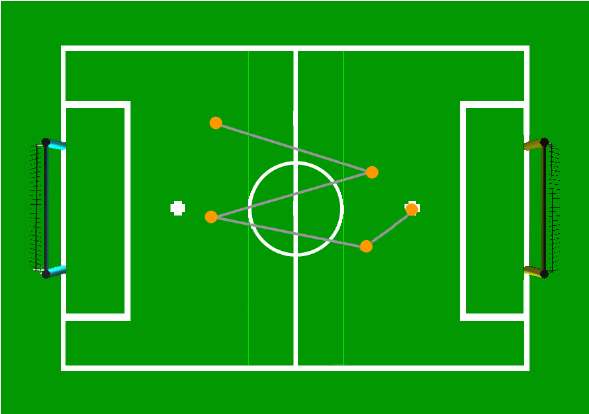
\includegraphics[width=0.75\textwidth]{figures/nao_passingchallenge.png}
 % nao_anyballchallenge.png: 791x564 pixel, 72dpi, 27.90x19.90 cm, bb=
 \caption{Setup and expectations for the Passing Challenge.}
 \label{fig:passingchallenge}
\end{figure}

The robots will have 3 minutes to perform 3 successive passes. The trial ends 
without success, that is the challenge ends, if the ball or one of the robots 
leaves the field, or if the ball stops inside the middle area or one of the 
robots enters the middle area. The ball is expected to cross the middle area 
3 times, as indicated by the example trajectory in Figure \ref{fig:passingchallenge}. 
The trial is considered successful if the receiving robot touches the ball after 
the third crossing.

Intermediate scoring for passing between robot 1 and 2 (robot 1 is the first kicking one):
\begin{itemize}
 \item $1^{st}$ touch of the ball to robot 2: 1 points
 \item $2^{nd}$ touch of the ball to robot 1: 2 points
 \item $3^{rd}$ touch of the ball to robot 2: 3 points
\end{itemize}

If a team completes the challenge successfully in less than 3 minutes, then the final 
placement among such teams will be based on how fast the challenge was completed.

\section{The Dribbling Challenge}
\label{sec:dribbling}

The dribbling challenge requires a combination of flexible ball manipulation and obstacle 
detection and avoidance skills. There will be three red robots on the field in their 
crouching goalie postures. The blocking robots will be placed on the field in such a way 
to prevent direct kicks towards the goal succeed; therefore, the dribbling robot needs to 
make sure that the path is clear before it attempts a kick. The dribbling robot will start 
from the front line of the penalty box of the blue goal and the ball will be placed on the 
cross mark in front of the robot. There is a total of three minutes for the robot to score 
a goal. The challenge ends with success if the dribbling robot is able to score without 
bumping into any of the stationary robots or the ball touching the blockers or going outside 
the field borders. Otherwise, the challenge ends without success. How much time the robot 
spent to score a goal will also be incorporated in the calculation of the final score.

\end{document}


